\documentclass[11pt]{article}
\usepackage{graphicx}
\usepackage[multiple]{footmisc}
\usepackage{cleveref}
\crefformat{footnote}{#2\footnotemark[#1]#3}
%Gummi|065|=)
\title{\textbf{Action selection - Guthrie Model}}
\author{Bhargav Teja Nallapu\\
		}
\date{}
\begin{document}

\maketitle

\section{Context}

This document refers to \emph{model}\footnote{http://www.labri.fr/perso/nrougier/downloads/ReproducibleScience.pdf} implemented by \emph{Meropi Topalidou}\footnote{\label{imn}Institute of Neurodegenerative Diseases - Bordeaux}\footnote{\label{inria}INRIA Bordeaux SUD-OUEST}, \emph{Arthur Leblois}\footnote{Laboratory of Neurophysics and Physiology Universite Paris Descartes}, \emph{Thomas boraud}\cref{imn}, \emph{Nicolas P. Rougier}\cref{imn}\cref{inria} 

The \emph{model} in its original version models action selection using an N-armed bandit task. With reference to Guthrie et al. (2013), the \emph{model} includes two distinct cognitive and motor loops to account for action selection at multiple levels. However the learning happens only in cognitive loop assuming that its the shape of the cue presented that matters to make a decision depending on the reward associated to it.

\section{Scenarios}
\subsection{Motor learning}
Here, we try to test, with motor learning in place, for different learning parameters, how the cognitive and motor weights (for directions) are learnt and how mean performance varies after various sessions.

\subsubsection{Cognitive learning, 250 sessions, 120 trials per session}
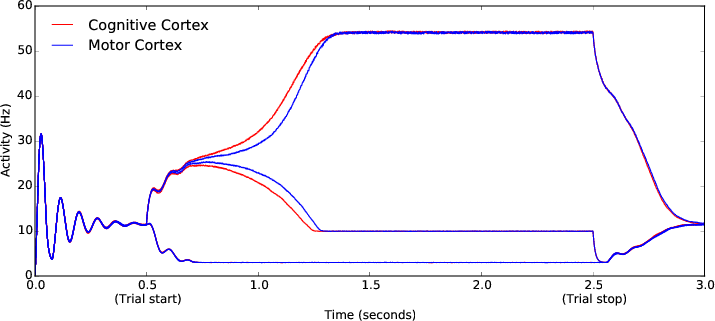
\includegraphics[scale=.6]{figure-1.png}
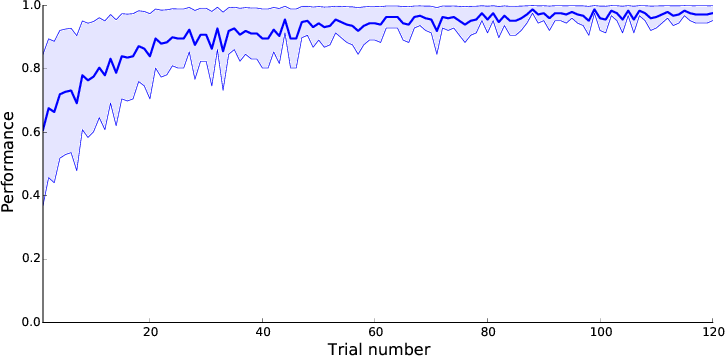
\includegraphics[scale=.5]{figure-2.png}

\subsubsection{Cognitive \& Motor learning, 250 sessions, 120 trials per session, standard learning rates}
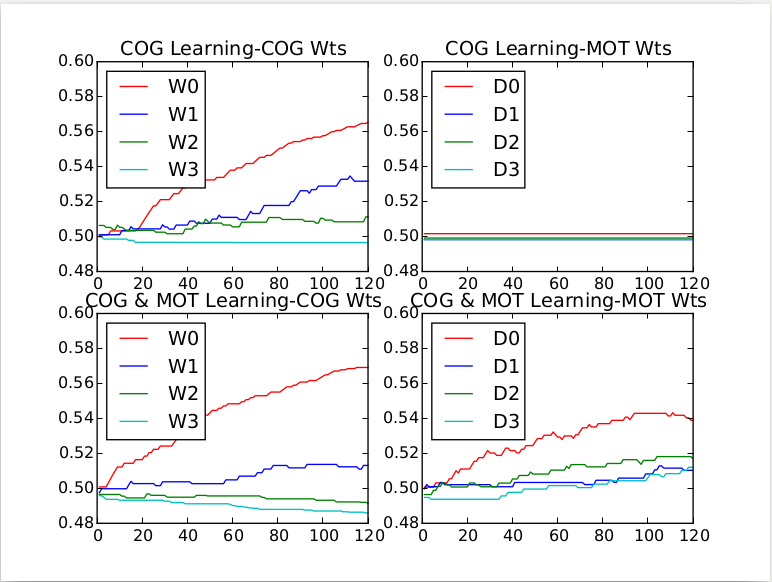
\includegraphics[clip=true, trim=15 15 0 15, scale=.5]{weights_same_rates.png}
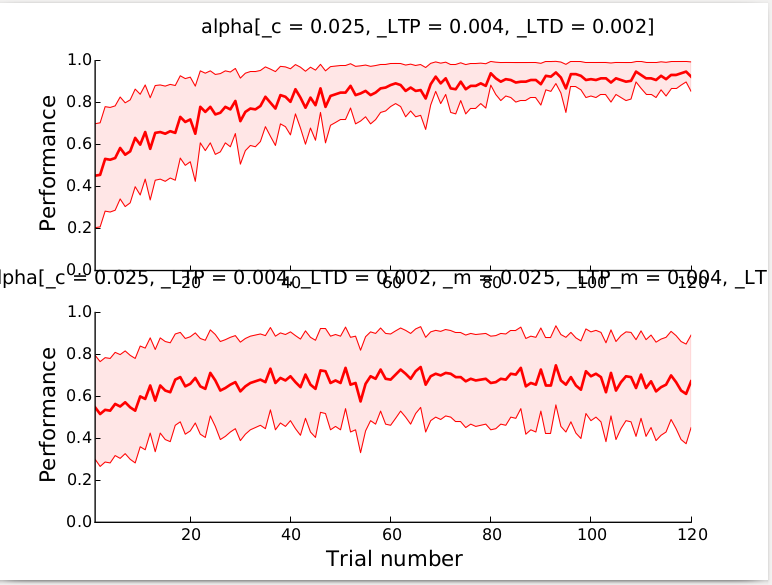
\includegraphics[clip=true, trim=15 15 0 15, scale=.5]{perf_same_rates.png}

\subsubsection{Cognitive \& Motor learning, 250 sessions, 240 trials per session, all learning rates cut by half when there is motor learning}
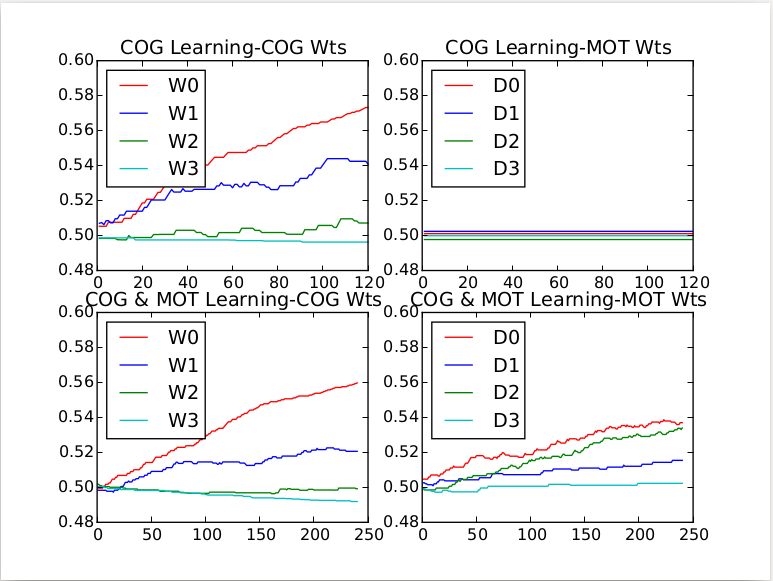
\includegraphics[clip=true, trim=15 15 0 15, scale=.5]{weights_diff_rates.png}
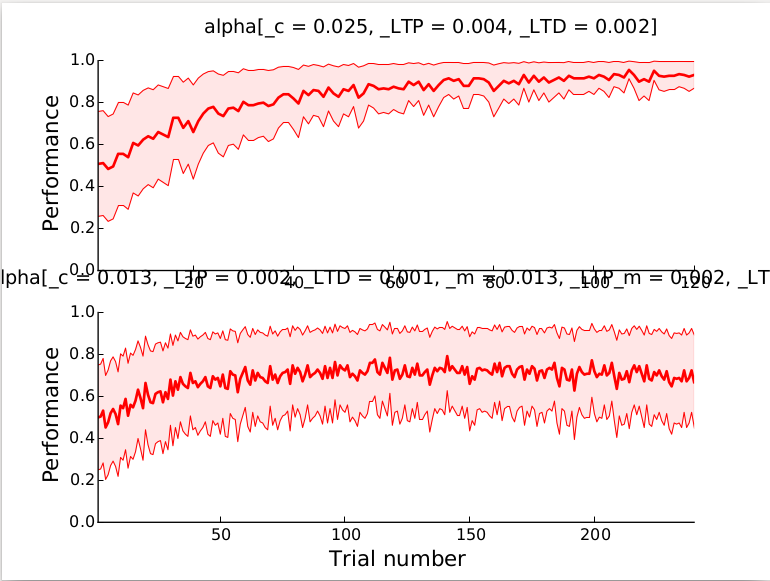
\includegraphics[clip=true, trim=15 15 0 15, scale=.5]{perf_diff_rates.png}

\subsection{Rewarding stimulus delayed}
In this scenario, of every possible combination of 2 cues, less rewarding cue is presented first. After a certain amount of delay, cue more rewarding than the first, is presented. This scenario is tested on a model which is already learnt and which has a performance nearly equal to 1 after learning. Each cue pair is presented 120 times, and mean performance is measured based on the cue selected.
\\
It is observed that the delay after which the best rewarding cue is not chosen varies with the difference of the reward probabilities of the two cues presented.
\subsubsection{Performance 120 trials/stimulus}
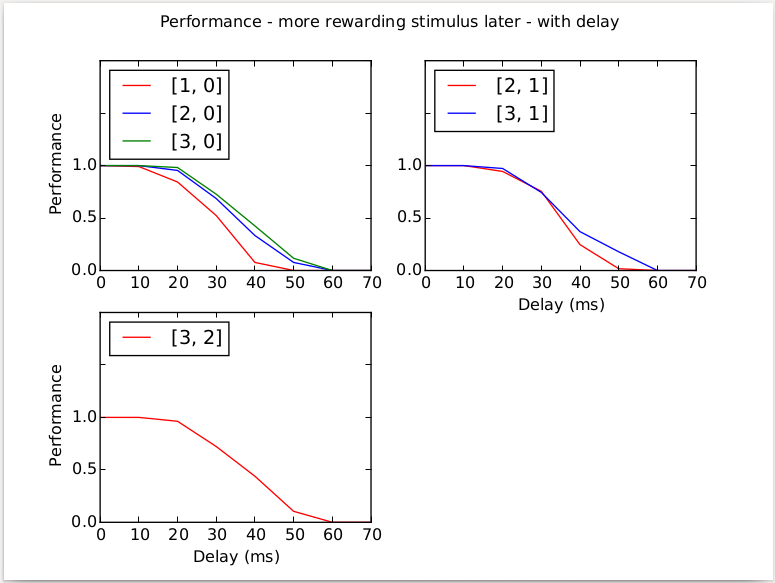
\includegraphics[clip=true, trim=25 35 0 35, scale=.7]{perf_with_delays.png}

\subsection{Less rewarding stimulus with higher salience}
In this scenario, we consider that a less rewarding (after having learnt) stimulus may be visually more appealing because of its salient features.Both the cues are presented simultaneously, but the less rewarding cue is presented with more salience. In the model, this is achieved by increasing the external input current to the cognitive input of the network corresponding to the less rewarding cue. 
\\
Similar to section 2.2, it is observed that the salience level after which the less rewarding cue is chosen over the best, varies with the difference of the reward probabilities of the two cues presented.
\subsubsection{Performance 120 trials/stimulus}
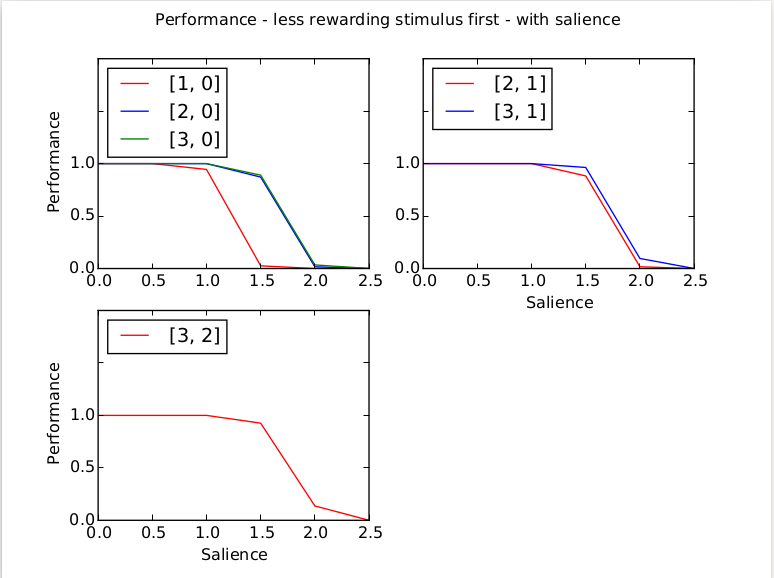
\includegraphics[clip=true, trim=25 35 0 35, scale=.7]{perf_with_salience.png}

\section{Week : 10-08-2015}
\subsection{Scaling up the model}
So far, the model represented each cue and each direction as a single unit which is a very simplified way of representation. To scale up the model, the idea is that a large number of \emph{neurons} encode each cue input and direction input. This refers to expanding the structures in the model such as the cognitive channels and motor channels in both cortex (CTX) as well as striatum (STR). Eventually the size of the associative channels in both CTX ans STR becomes very large.\par
The cue input presentation is chosen as a gaussian input over the sub-group of \emph{neurons} representing paricular cue. The output is expected to be a similar activation, but only in the sub-group of neurons representing the desired cue output.\\
\par
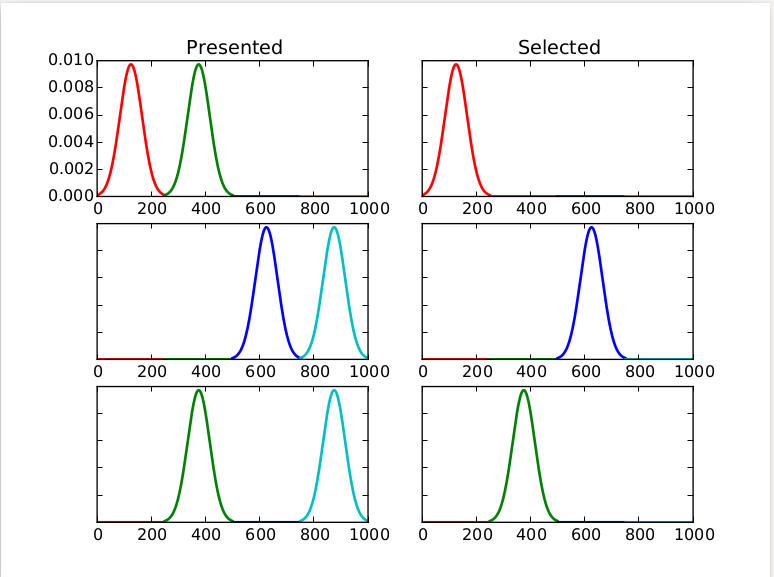
\includegraphics[clip=true, trim=40 35 0 35, scale=.5]{pop_inputs.png}
\subsection{TBD next week}
The plan is to identify all the channels and structures in the model which can be scaled from a simplified representation to a more realistic population of neurons
\end{document}
